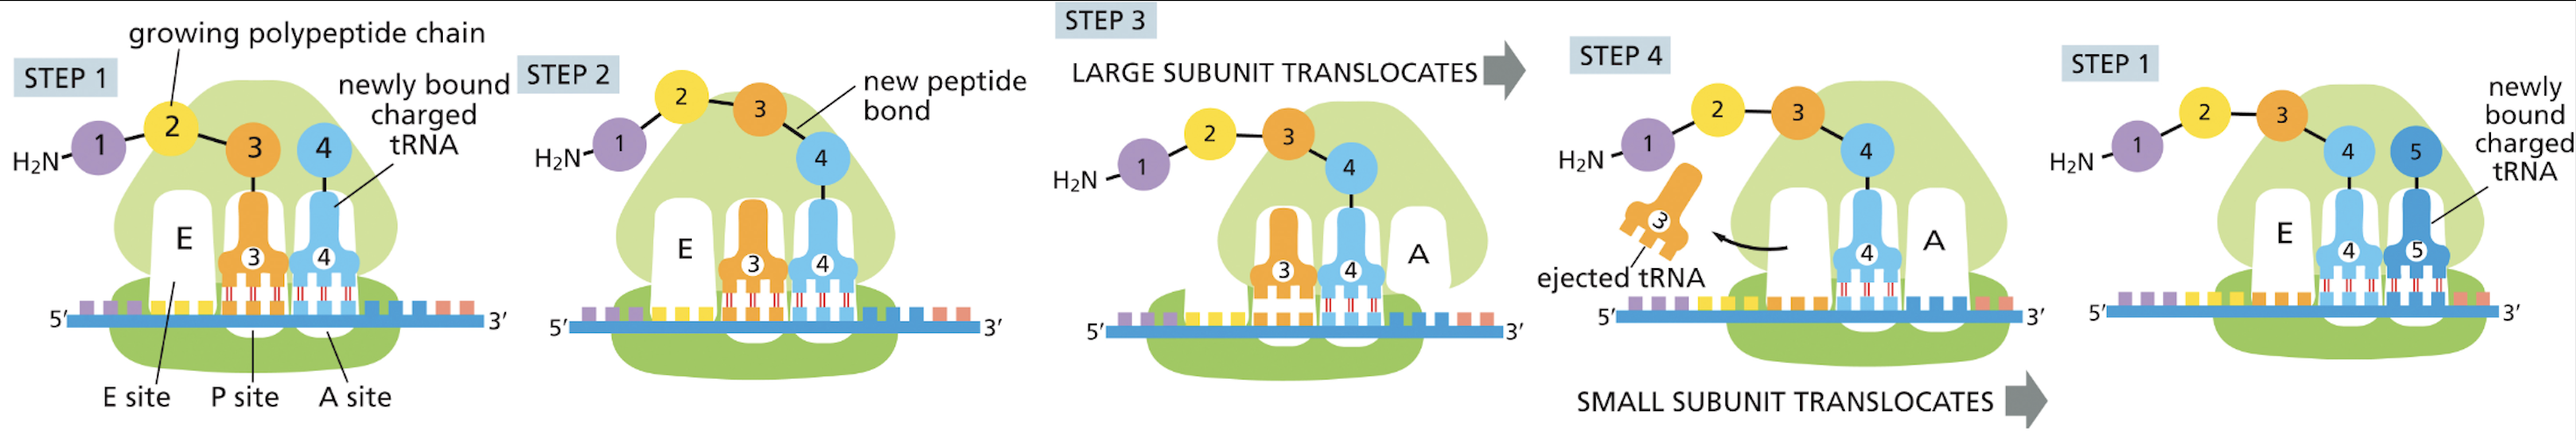
\includegraphics[width=70mm]{src/Images/translation_ribosome.png}\\ 
\begin{itemize}
    \item On the mRNA, every three bases (= nucleotides) form one codon (needs ATP).
    \item A tRNA brings a matching amino acid. It has an anticodon that is complementary to the mRNA codon.
    \item The tRNA binds to the mRNA in the ribosome (at the A site).
    \item The amino acid is added to the growing polypeptide chain.
    \item The tRNA is ejected (from the E site), and the ribosome shifts forward by one codon.
    \item The process repeats until a stop codon is reached.
\end{itemize}
Multiple ribosomes can translate the same mRNA at the same time (making multiple proteins at the time), forming a polyribosome (or polysome).






